\documentclass[tikz,border=2pt]{standalone}
\usepackage{amsmath,amssymb}
\usepackage{tikz}
\usetikzlibrary{arrows.meta,matrix}

\begin{document}
% Cofactor expansion along the first row: each entry times the sign (-1)^{i+j} times the
% determinant of what is left after deleting its row and column.
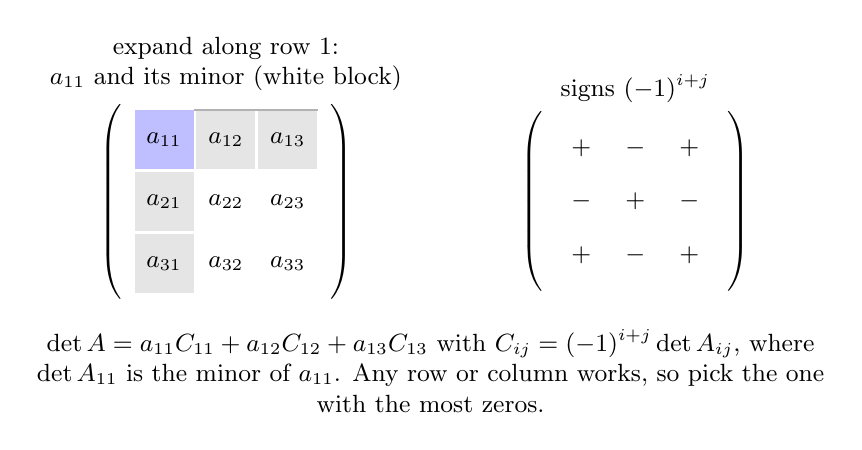
\begin{tikzpicture}[every node/.style={font=\small}]
	\matrix (A) [matrix of math nodes, nodes={minimum size=7.5mm, anchor=center}, left delimiter=(, right delimiter=), column sep=1pt, row sep=1pt] at (0,0) {
		|[fill=blue!25]| a_{11} & |[fill=gray!20]| a_{12} & |[fill=gray!20]| a_{13} \\
		|[fill=gray!20]| a_{21} & a_{22} & a_{23} \\
		|[fill=gray!20]| a_{31} & a_{32} & a_{33} \\
	};
	\draw[gray!60, thick] (A-1-1.north east) -- (A-1-3.north east);
	\node[anchor=south, font=\small, align=center] at (A.north) {expand along row $1$:\\ $a_{11}$ and its minor (white block)};
	\matrix (S) [matrix of math nodes, nodes={minimum size=6.5mm, anchor=center}, left delimiter=(, right delimiter=), column sep=1pt, row sep=1pt] at (5.2,0) {
		+ & - & + \\
		- & + & - \\
		+ & - & + \\
	};
	\node[anchor=south, font=\small] at (S.north) {signs $(-1)^{i+j}$};
	\node[anchor=north, align=flush center, text width=10cm] at (2.6,-1.5) {$\det A=a_{11}C_{11}+a_{12}C_{12}+a_{13}C_{13}$ with $C_{ij}=(-1)^{i+j}\det A_{ij}$, where $\det A_{11}$ is the minor of $a_{11}$. Any row or column works, so pick the one with the most zeros.};
\end{tikzpicture}
\end{document}
